\section{Background}
\label{sec:sec001}
It has always been hard, if not impossible, to monitor and keep track of animals' pattern~\cite{gibb2018emerging}.
Knowing animal's patterns will greatly improve livestock production~\cite{eldridge2016new, clink2017investigating}.
Traditional livestock monitoring methods are limited by being resource intensive and invasive.
This then led to an improving need on the field of livestock monitoring methods.
In this regard, the idea of acoustically monitoring animals (Figure \ref{fig:img002}) came up.
As a matter of fact, animal acoustical monitoring allow continuous remote data collection, and can serve productions across an inexpensive assemble collar for device recording.
Therefore, it is a viable method for characterizing animal productions.

%%%%%%%%%%%%%%%%%%%%%%%%%%%%%%%%%%%%%%%%%%%%%%%%%%

\hfill

\begin{figure}[!ht]
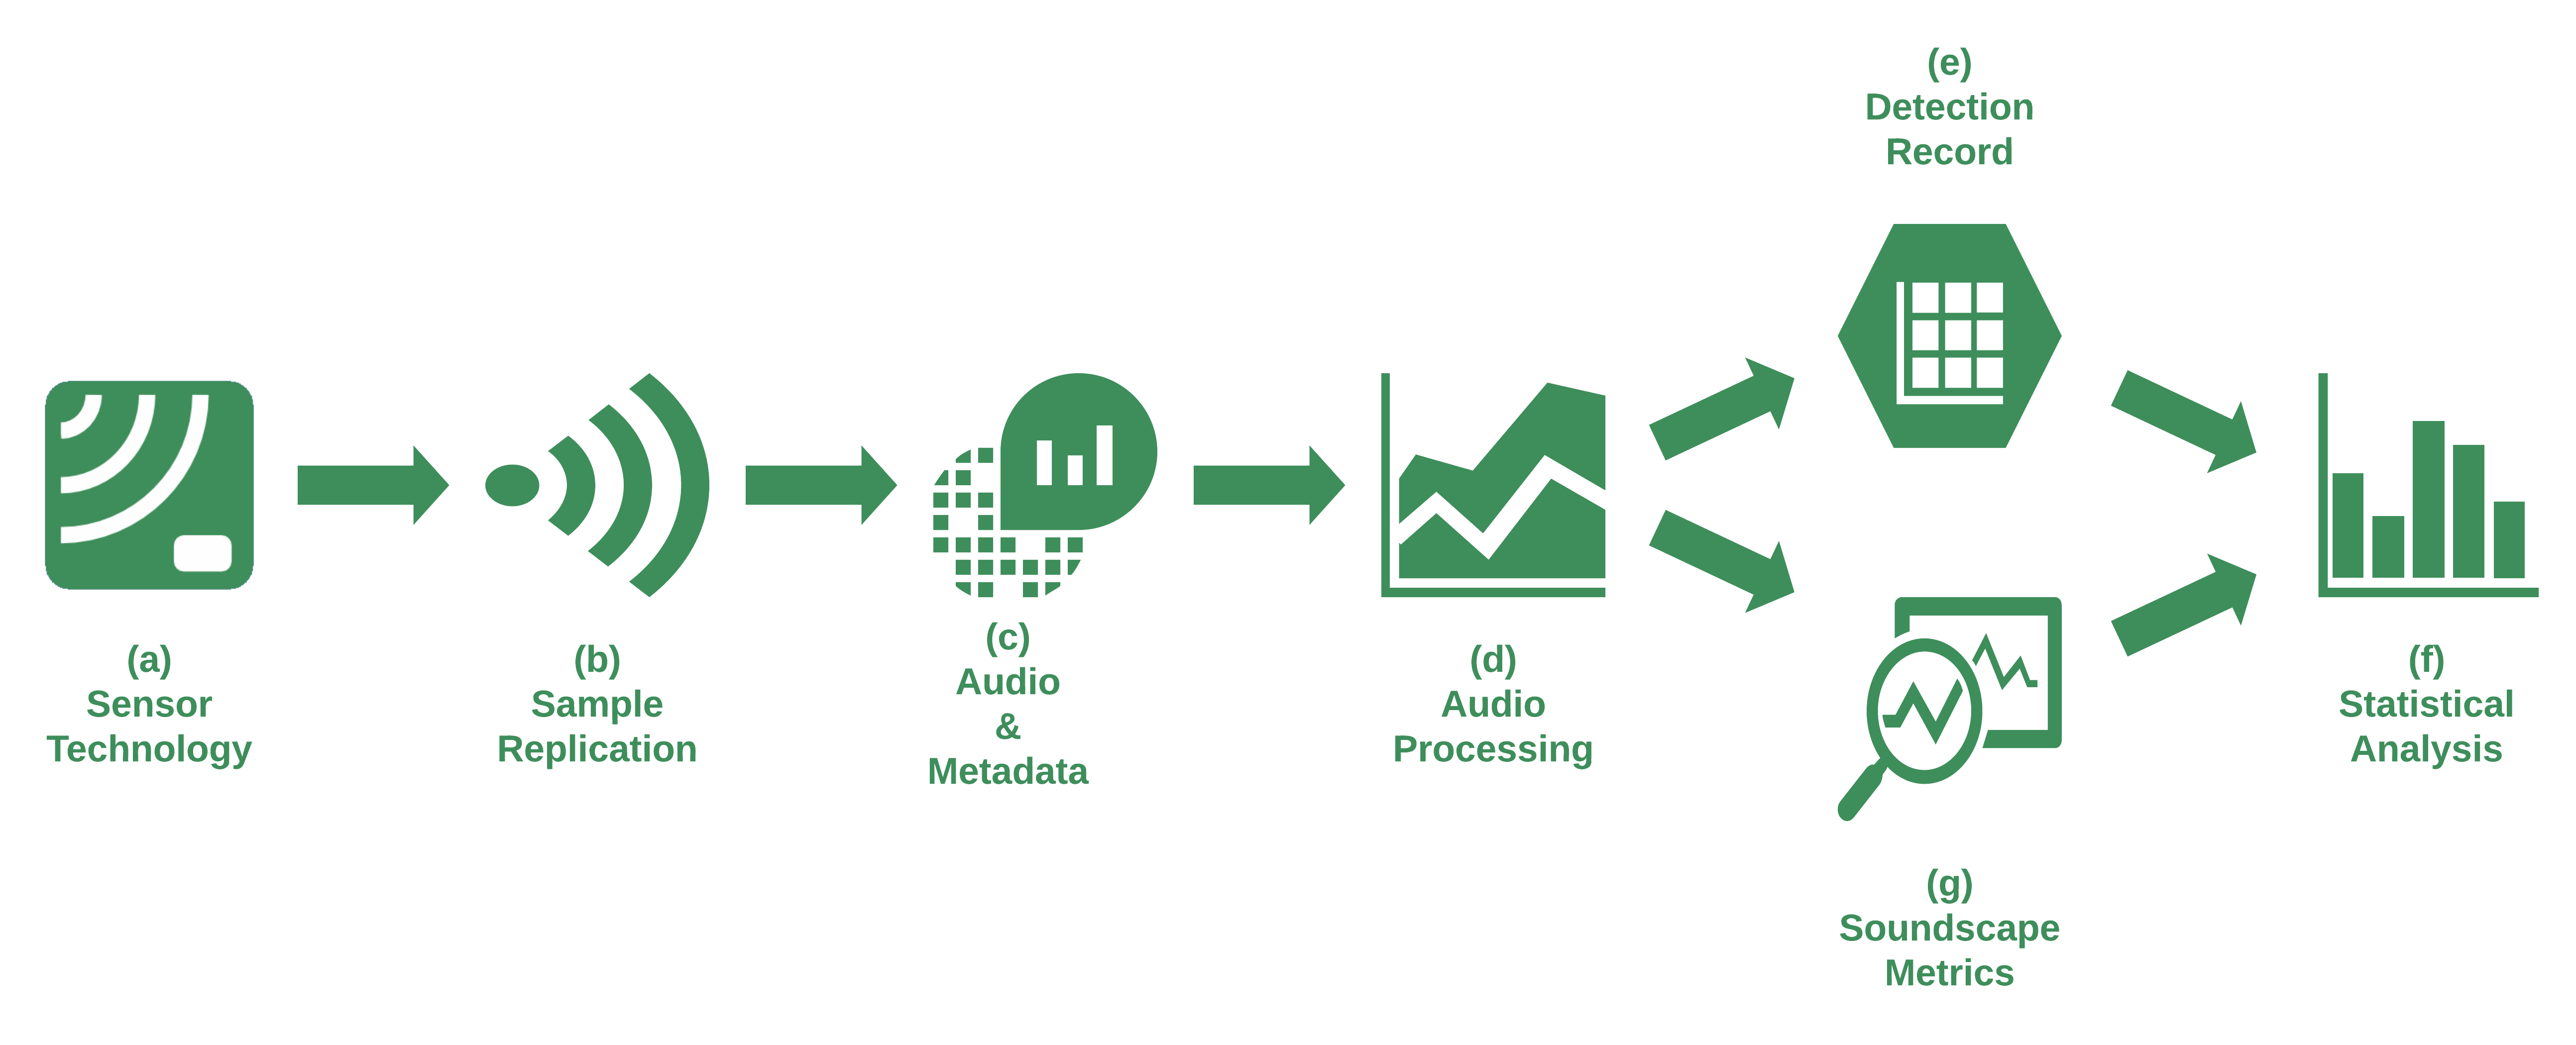
\includegraphics[width=\columnwidth]{img002}
\caption{Passive Acoustic Monitoring (PAM) workflow proposal. Pipeline for the current application of PAM technologies, to identify challenges and research priorities at each stage. The Figure show each stage of the process regarding potential use of the (a) Sensor Technology (\textit{AudioMoth}).}
\label{fig:img002}
\end{figure}

\hfill

%%%%%%%%%%%%%%%%%%%%%%%%%%%%%%%%%%%%%%%%%%%%%%%%%%

Passive acoustic sensors have become an increasingly potential for animal monitoring.
Many animals emit acoustic signals that encode information regarding their presence, health condition and activities~\cite{bradbury1998principles}.
However, opportunities to acoustically examine livestock productions have historically been limited by technological constrains and costs.
This situation is fast improving.
For instance, the release of \textit{AudioMoth}~\cite{hill2018audiomoth}, as a low-cost sensor, has seen broad uptake for study goals at ranging from population control to activity state~\cite{jones2013indicator, newson2015novel}.

The passive acoustic approaches have long been applied to monitor visually cryptic livestock productions such as sheep, cow and pig breeding~\cite{frost1997review}.
These established acoustic examination methods typically involves livestock counting to identify each animal on a herd.
This process, is done by moving the herd to an animal sleeve, counting one by one.
But, in recent years, their scopes has expanded with the arrival of novel proposed acoustic sensors.

The proposed use of acoustic sensors make possible of sensing technologies.
Many animals actively produce sound for communication.
Also, typical livestock species emit sounds that can be labelled, enabling to create a complete dataset~\cite{tullo2013precision}.
This dataset is suitable for algorithm development, thus leading to the development of \hyperlink{http://www.sa-instrumentation.com/technology/}{Passive Acoustic Monitoring (PAM)}~\cite{zimmer2011passive}.

The PAM involves recording sound using passive acoustic sensors (Figure \ref{fig:img002}), like \textit{AudioMoth}, and subsequently deriving relevant data from audio (e.g., counting number of animals, epidemic situations and animal events).
Vocalising animals can leak information into their surrounding regarding their behaviour, presence and interactions in time and space~\cite{kershenbaum2016acoustic}.